\section{Systemtechnik}
\subsection{Modellbildung}
Hinweise zum aufstellen der Differentialgleichung eines Systems:
\begin{mdframed}[style=exercise]
	\begin{enumerate}
		\item Bestimmung der Ein- und Ausgangsgrößen
		\item Suche nach dem beschreibenden Gleichgewicht
		\item In der Gleichung dürfen nur Konstanten, sowie die Ein- und
		      Ausgangsgrößen in beliebiger Ableitung vorkommen
		\item Andere Variablen müssen durch erlaubte Größen ersetzt werden\\
		      \footnotesize
		      (Dazu können i.a. physikalische Gleichungen benutzt werden)
	\end{enumerate}
\end{mdframed}

\subsection{Signalflussplan/Blockschaltbild}
Erzeugung des Signalflussplans aus der Zugehörigen DGL.
\begin{mdframed}[style=exercise]
	\begin{enumerate}
		\item für technische Realisierung gilt: m < n;

		\item DGL. nach höchster Ableitung der Ausgangsgröße auflösen

		\item höchste Ableitung der Ausgangsgröße geht auf den Eingang des ersten Integrators\\
		      \footnotesize
		      (Laplace-Trans ersetzt das Integrieren mit einer Division mit „s“)
	\end{enumerate}
\end{mdframed}
\begin{center}
	\includegraphics[width=0.96\columnwidth]{Figures/Signalflussplan12.png}
\end{center}

Erzeugung des Signalflussplans eines Systems mit der DGL.:

\begin{align*}
	  & a_{n} \overset{(n)}{x}_{a}+\ldots+a_{2} \ddot{x}_{a}+a_{1} \dot{x}_{a}+a_{0} x_{a} \\
	= & b_{n} \overset{(n)}{x}_{e}+\ldots+b_{2} \ddot{x}+b_{1} \dot{x}_{e}+b_{0} x_{e}
\end{align*}

Signalflussplan kann allgemein gezeichnet werden: (nötig, falls eine Ableitung von $x_e$ existiert)

\includegraphics[width=0.9\columnwidth]{Figures/SFmitDGL.png}

\subsection{Stabilität}
\begin{mdframed}[style=exercise]
	BIBO-Stabilität (Bounded Input/ Bounded Output-> begrenzt):\\
	ein dynamisches System ist stabil, wenn gilt:\\
	für ein begrenztes $x_e$ gibt es immer ein begrenztes $x_a$
\end{mdframed}

\subsection{Ortskurven und Frequenzkennlinien}

Ortskurvendarstellung:
\begin{center}
	\includegraphics[width=0.96\columnwidth]{Figures/Ortskurve.png}
\end{center}
\begin{mdframed}[style=exercise]
	Für wachsendes $\omega$ werden die komplexen Werte F(j$\omega$) in die
	komplexe F-Ebene eingetragen und zur Ortskurve verbunden.\\ Jeder
	Ortskurvenpunkt kann jetzt als Zeiger gedeutet werden.
\end{mdframed}

\newpage
Bodediagramm Darstellung:
\begin{center}
	\includegraphics[width=0.96\columnwidth]{Figures/Bodediagramm.png}
\end{center}
\begin{mdframed}[style=exercise]
	Der Amplitudengang A($\omega$) wird in doppelt logarithmischer Darstellung
	aufgetragen,\\ der Phasengang y($\omega$)) halblogarithmisch. Gemeinsame
	Abszisse ist $\omega$.

	Bei diesem Beispiel (PT1-Glied) ist deutlich der\\ Tiefpass-Charakter zu
	erkennen.

	Verkettete Funktionen im Bodediagramm resultieren als Produkt der
	Einzelübertragungsfunktionen.

	D.h. Verstärkung wird multipliziert und Phasenverschiebung addiert.\\ Das
	heißt: Sowohl Phasengang (halblogarithmische Darstellung) und Amplitudengang
	(logarithmische Darstellung) werden graphisch addiert!
\end{mdframed}

\subsection{$\mathbf{F(s)}$ in Pol- und Nullstellenform}
\begin{mdframed}[style=exercise]
	Zähler- und Nennerpolynom von F(s) besitzt Nullstellen. Diese sind von
	$a_v$ und $b_u$ abhängig.\\
	Nullstellen des Zählers sind Nullstellen von F(s)\\
	Nullstellen des Nenners sind Polstellen von F(s)\\
	Wenn Pole $s_pv$ und Nullstellen $s_nu$ bekannt, kann man F(s) mit dem
	Faktor Q in faktorisierter Form darstellen.
\end{mdframed}

\[
	F(s)=Q \cdot \frac{\prod_{\mu=1}^{m}\left(s-s_{N \mu}\right)}{\prod_{v=1}^{n}\left(s-s_{P V}\right)}
	\qquad \texttt{mit } Q = \frac{b_m}{a_n}
\]

\begin{mdframed}[style=exercise]
	Die Stabilität von $F(s)$ kann anhand der Lage der Pole $s_pv$ in der s-Ebene
	beurteilt werden.\\ $F(s)$ ist stabil, wenn alle Pole $s_pv$ in der linken
	s-Halbebene liegen.\\ Instabile Pole in der Rechten Halbebene lassen sich
	nicht durch Reihenschaltung mit entsprechender Nullstelle kompensieren!
\end{mdframed}
\begin{mdframed}[style=exercise]
	Bedeutung Polstelle:

	Pole bewirken ein zeitverzögertes Verhalten. Je weiter links sie sich befinden,
	desto schneller ist der Einschwingvorgang.

	$\Rightarrow$ Wenn Pole deutlich weiter links liegen als andere andere, kann man sie ohne
	großen Fehler vernachlässigen.
\end{mdframed}
\begin{mdframed}[style=exercise]
	Bedeutung Nullstelle:\\
	NS bewirken ein differenzierendes Verhalten (Beschleunigung des Systems)
	Einfluss weit links in der s-Ebene kann häufig vernachlässigt werden.

\end{mdframed}

\subsection{Signalflussplan Algebra}
\begin{itemize}[leftmargin=*]
	\item Kettenstruktur:
	      \begin{center}
		      \includegraphics[width=0.96\columnwidth]{Figures/Kettenstruktur.png}
	      \end{center}

	\item Parallelstruktur:
	      \begin{center}
		      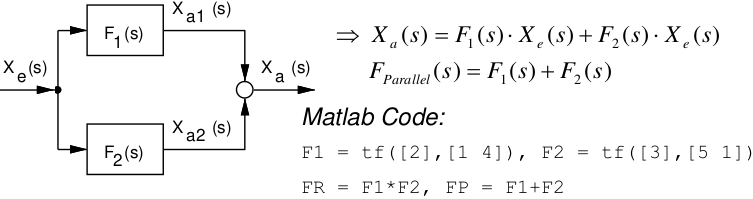
\includegraphics[width=0.96\columnwidth]{Figures/Parallelstruktur.png}
	      \end{center}

	\item Kreisstruktur:
	      \begin{center}
		      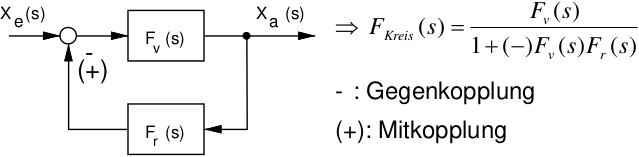
\includegraphics[width=0.96\columnwidth]{Figures/Kreisstruktur.png}
	      \end{center}

	\item Verschieben einer Additionsstelle:
	      \begin{center}
		      \includegraphics[width=0.9\columnwidth]{Figures/Verschiebung einer Additionsstelel.png}
	      \end{center}

	\item Verschieben einer Verzweigung:
	      \begin{center}
		      \includegraphics[width=0.9\columnwidth]{Figures/Verschiebung einer Verzweigung.png}
	      \end{center}
\end{itemize}
